\section{Auswertung}
\label{sec:Auswertung}

\subsection{Bestimmung der Zeitkonstante eines RC-Glieds}
Die Abbildung \ref{fig:entladung} zeigt die Entladekurve des RC-Glieds.
In Tabelle \ref{tab:entladung} ist die Spannung $U_\text{c}$ zum Zeitpunkt $t$ aufgelistet.
Die angelegte Spannung beträgt $U_0 = \SI{0.5}{\volt}$. Im Folgenden werden drei Methoden
zur Berechnung der Zeitkonstante $RC$ aufgeführt.
\begin{figure}
    \centering
    \includegraphics[width=\textwidth]{content/data/entlade.jpg}
    \caption{Entladekurve eines RC-Glieds mit einem Oszilloskop gemessen.}
    \label{fig:entladung}
\end{figure}
\begin{table}
    \centering
    \begin{tabular}{cc|cc}
        \toprule
        $t\,/\,\si{\milli\second}$ & $U_\text{c}\,/\,V$ & $t\,/\,ms$ & $U_\text{c}\,/\,V$ \\ 
        \midrule
        0.0 & 0.54 & 1.2 & 0.12 \\
        0.1 & 0.48 & 1.3 & 0.10 \\
        0.2 & 0.42 & 1.4 & 0.08 \\
        0.3 & 0.38 & 1.5 & 0.07 \\
        0.4 & 0.33 & 1.6 & 0.06 \\
        0.5 & 0.30 & 1.7 & 0.05 \\
        0.6 & 0.26 & 1.8 & 0.04 \\
        0.7 & 0.22 & 1.9 & 0.03 \\
        0.8 & 0.20 & 2.0 & 0.02 \\
        0.9 & 0.17 & 2.1 & 0.02 \\
        1.0 & 0.15 & 2.2 & 0.01 \\
        1.1 & 0.13 & 2.3 & 0.01 \\
        \bottomrule
    \end{tabular}
    \caption{Messwerte einer Entladekurve in einem RC-Kreis.}
    \label{tab:entladung}
\end{table}
\FloatBarrier

\subsubsection{Methode 1: lineare Ausgleichsrechnung}
Mithilfe der linearen Ausgleichsrechnung kann die Steigung der Geraden $a$ und die Zeitkonstante $RC=-\frac{1}{a}$ bestimmt werden.
Für die Geradengleichung
\begin{equation}
    \ln U_\text{c}(t) = a \cdot t + b
    \label{eqn:gerade}
\end{equation}
ergeben sich die Parameter
\begin{equation*}
    RC = \SI{0.5969(229)}{\milli\second}
\end{equation*}
\begin{equation*}
    b = \SI{-0.35887(863)} .
\end{equation*}
In Abbildung \ref{fig:plota} sind die Messwerte und die Gerade \ref{eqn:gerade} aufgetragen.
\begin{figure}
    \centering
    \includegraphics[width=\textwidth]{content/data/plota.pdf}
    \caption{Lineare Ausgleichsrechnung und Messwerte eines RC-Glieds im Vergleich.}
    \label{fig:plota}
\end{figure}
\FloatBarrier

\subsubsection{Methode 2: Ausgleichsrechnung über Kondensatorspannung}
In Tabelle \ref{tab:phase} ist die Amplitude der Kondensatorspannung $U_\text{c}$ und die Phasenverschiebung $\varphi$ in Abhängigkeit von der Frequenz $f$ aufgelistet.
\begin{table}
    \centering
    \begin{tabular}{ccccc}
    \toprule
    $f\,/\,\si{\hertz}$ & $U_\text{c} \,/\, \si{\volt}$ & $a\,/\,\si{\milli\second}$ & $b\,/\,\si{\milli\second}$ & $\varphi \,/\,rad$ \\
    \midrule
    20 & 0.600 & 1.000 & 36.00 &0.17453293\\
    30 & 0.600 & 1.000 & 24.00 &0.26179939\\
    40 & 0.580 & 0.900 & 18.00 &0.31415927\\
    50 & 0.570 & 0.900 & 14.60 &0.38731964 \\
    60 & 0.560 & 0.900 & 12.20 &0.46351367 \\
    70 & 0.520 & 0.850 & 10.40 &0.51352957\\
    80 & 0.520 & 0.850 & 9.20  &0.58051169 \\
    90 & 0.500 & 0.800 & 8.20  &0.61299369 \\
    100 & 0.480 & 0.800 & 7.20 &0.6981317  \\
    200 & 0.320 & 0.580 & 3.60 &1.01229097 \\
    300 & 0.230 & 0.440 & 2.40 &1.15191731 \\
    400 & 0.180 & 0.360 & 1.80 &1.25663706\\
    500 & 0.145 & 0.300 & 1.44 &1.30899694 \\
    600 & 0.120 & 0.255 & 1.20 &1.33517688 \\
    700 & 0.105 & 0.225 & 1.04 &1.35934298 \\
    800 & 0.090 & 0.200 & 0.90 &1.3962634  \\
    900 & 0.082 & 0.180 & 0.80 &1.41371669 \\
    1000 & 0.074 & 0.164 & 0.7 &1.43116999\\
    2000 & 0.037 & 0.085 & 0.3 &1.48352986 \\
    3000 & 0.0185 & 0.058 & 0.24&1.51843645 \\
    4000 & 0.0110 & 0.044 & 0.18&1.53588974 \\
    6000 & 0.0075 & 0.0285 & 0.12&1.49225651 \\
    8000 & 0.0054 & 0.0225 & 0.09&1.57079633 \\
    10000 & 0.0044 & 0.0180 & 0.07&1.57079633\\
    20000 & 0.0021 & 0.0092 & 0.0365&1.58370698 \\
    30000 & 0.0014 & 0.0063 & 0.0245&1.61567622\\
    \bottomrule
    \end{tabular}
    \caption{Phasenverschiebung $\varphi$ und Kondensatorspannung $U_\text{c}$ in Abhängigkeit der Frequenz $f$ in einem RC-Glied.}
    \label{tab:phase}
\end{table}
Methode 2 verwendet die nicht-lineare Ausgleichsrechnung.
Dabei wird die Gleichung \ref{eqn:ampli}, welche die Beziehung zwischen Kondensatorspannung $U_\text{c}$ und der Kreisfrequenz $\omega = 2 \pi f$ beschreibt, verwendet.
Der Generator generiert eine Sinusspannung mit der Amplitude $U_0 = \SI{0.6}{\volt}$.
Mit der nicht-linearen Ausgleichsfunktion
\begin{equation}
    \frac{U_\text{c}}{U_0} = \frac{1}{\sqrt{1+w^2(RC)^2}}
    \label{eqn:nichtlin}
\end{equation}
ergibt sich für den Zeitparameter
\begin{equation*}
    RC = \SI{1.2360(167)}{\milli\second} .
\end{equation*}
In Abbildung \ref{fig:spannung} ist die Funktion \ref{eqn:nichtlin} mit der ermittelten Zeitkonstante $RC$ in einem halblogarithmischen Diagramm aufgetragen.
Zudem sind die Messwerte zum Vergleich eingetragen.
\begin{figure}
    \centering
    \includegraphics[width=\textwidth]{content/data/plotb.pdf}
    \caption{Das Verhältnis von Kondensatorspannung $U_\text{c}$ zu $U_0$ in Abhängigkeit der Frequenz $f$ in einem halblogarithmischen Diagramm.}
    \label{fig:spannung}
\end{figure}
\FloatBarrier

\subsubsection{Methode 3: Ausgleichsrechnung über die Phasenverschiebung}
Methode 3 verwendet die Phasenverschiebung $\varphi = \frac{a}{b}2\pi$ um $RC$ zu ermitteln.
Die Ausgleichsfunktion
\begin{equation}
    \varphi = \arctan(-\omega RC)
    \label{eqn:nlinphase}
\end{equation}
folgt aus der Beziehung von $\varphi$ und $\omega$ (siehe Gleichung \ref{eqn:phase}).
Wobei die Beziehung $\omega = 2\pi f$ verwendet wird.
Für $RC$ ermittelt über die Phasenverschiebung zwischen Kondensator und RC-Glied, ergibt sich
\begin{equation*}
    RC = \SI{1.2685(214)}{\milli\second} .
\end{equation*}
In dem halblogarithmischen Diagramm (Abb. \ref{fig:phase}) ist die Funktion \ref{eqn:nlinphase} und die gemessene Phase $\varphi$ aufgetragen.
Mithilfe der Daten aus Tabelle \ref{tab:phase} erhalten wir den Polarplot (Abb. \ref{fig:polar}) mit der theoretischen Kurve und den Messwerten $(\varphi, \frac{U_\text{c}}{U_0})$.
\begin{figure}
    \centering
    \includegraphics[width=\textwidth]{content/data/plotc.pdf}
    \caption{Die Phasenverschiebung $\varphi$ in Abhängigkeit der Frequenz $f$ in einem halblogarithmischen Diagramm.}
    \label{fig:phase}
\end{figure}

\begin{figure}
    \centering
    \includegraphics[width=\textwidth]{content/data/plotd.pdf}
    \caption{Abhängigkeit der Relativamplitude $A(\omega)/U_0$ von der Phase $\varphi$ in einem Polarkoordinatensystem.}
    \label{fig:polar}
\end{figure}
\FloatBarrier

\subsection{RC-Kreis als Integrator}
    In der Abbildung \ref{fig:integrabel} ist zu erkennen, dass der RC-Kreis für hohe Frequenzen $\omega >> 1/RC$ als Integrator arbeitet.
    Hier wird eine Frequenz von $\SI{45}{\kilo\hertz}$ verwendet.
    Die veränderte Spannung kann nach Gleichung \ref{eqn:integrator} berechnet werden (siehe Tab. \ref{tab:integration}).
    \begin{figure}
        \centering
        \begin{subfigure}[b]{0.475\textwidth}
            \centering
            \includegraphics[width=\textwidth]{content/data/sinus.jpg}
            \caption[Network2]%
            {{\small Sinusschwingung}}    
            \label{fig:mean and std of net14}
        \end{subfigure}
        \hfill
        \begin{subfigure}[b]{0.475\textwidth}  
            \centering 
            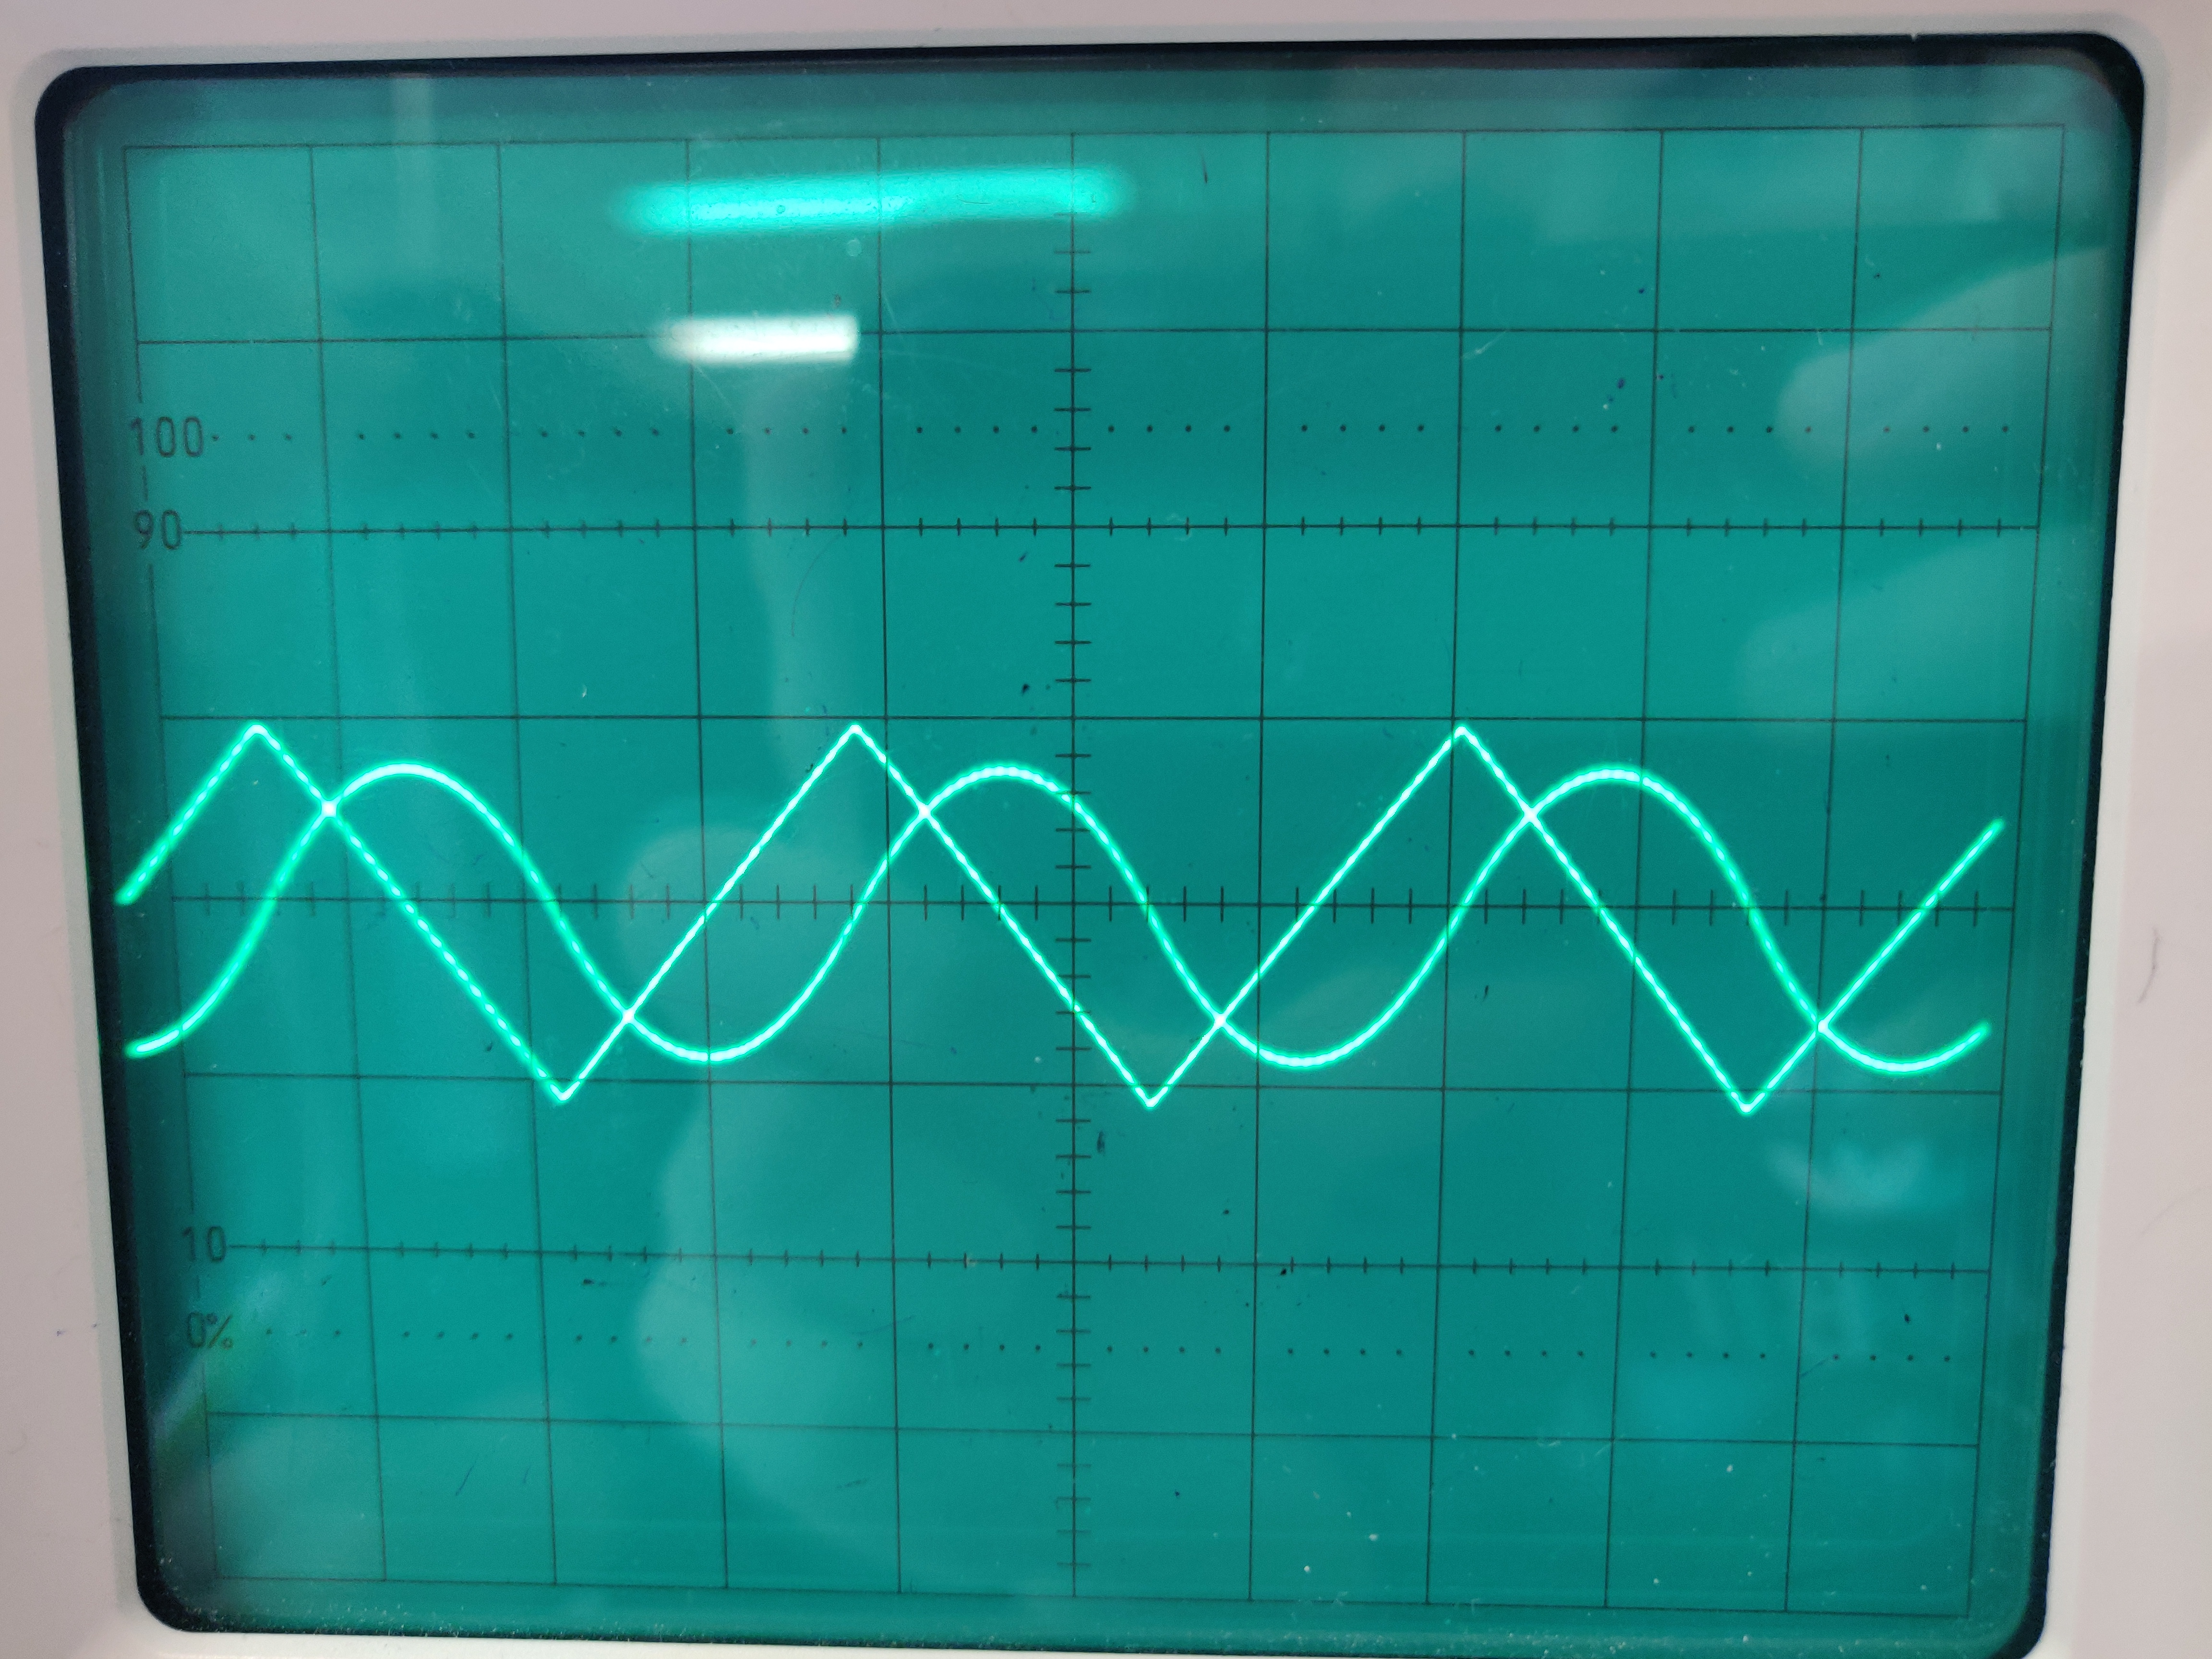
\includegraphics[width=\textwidth]{content/data/dreieck.jpg}
            \caption[]%
            {{\small Dreiecksschwingung}}    
            \label{fig:mean and std of net24}
        \end{subfigure}
        \vskip\baselineskip
        \begin{subfigure}[b]{0.475\textwidth}   
            \centering 
            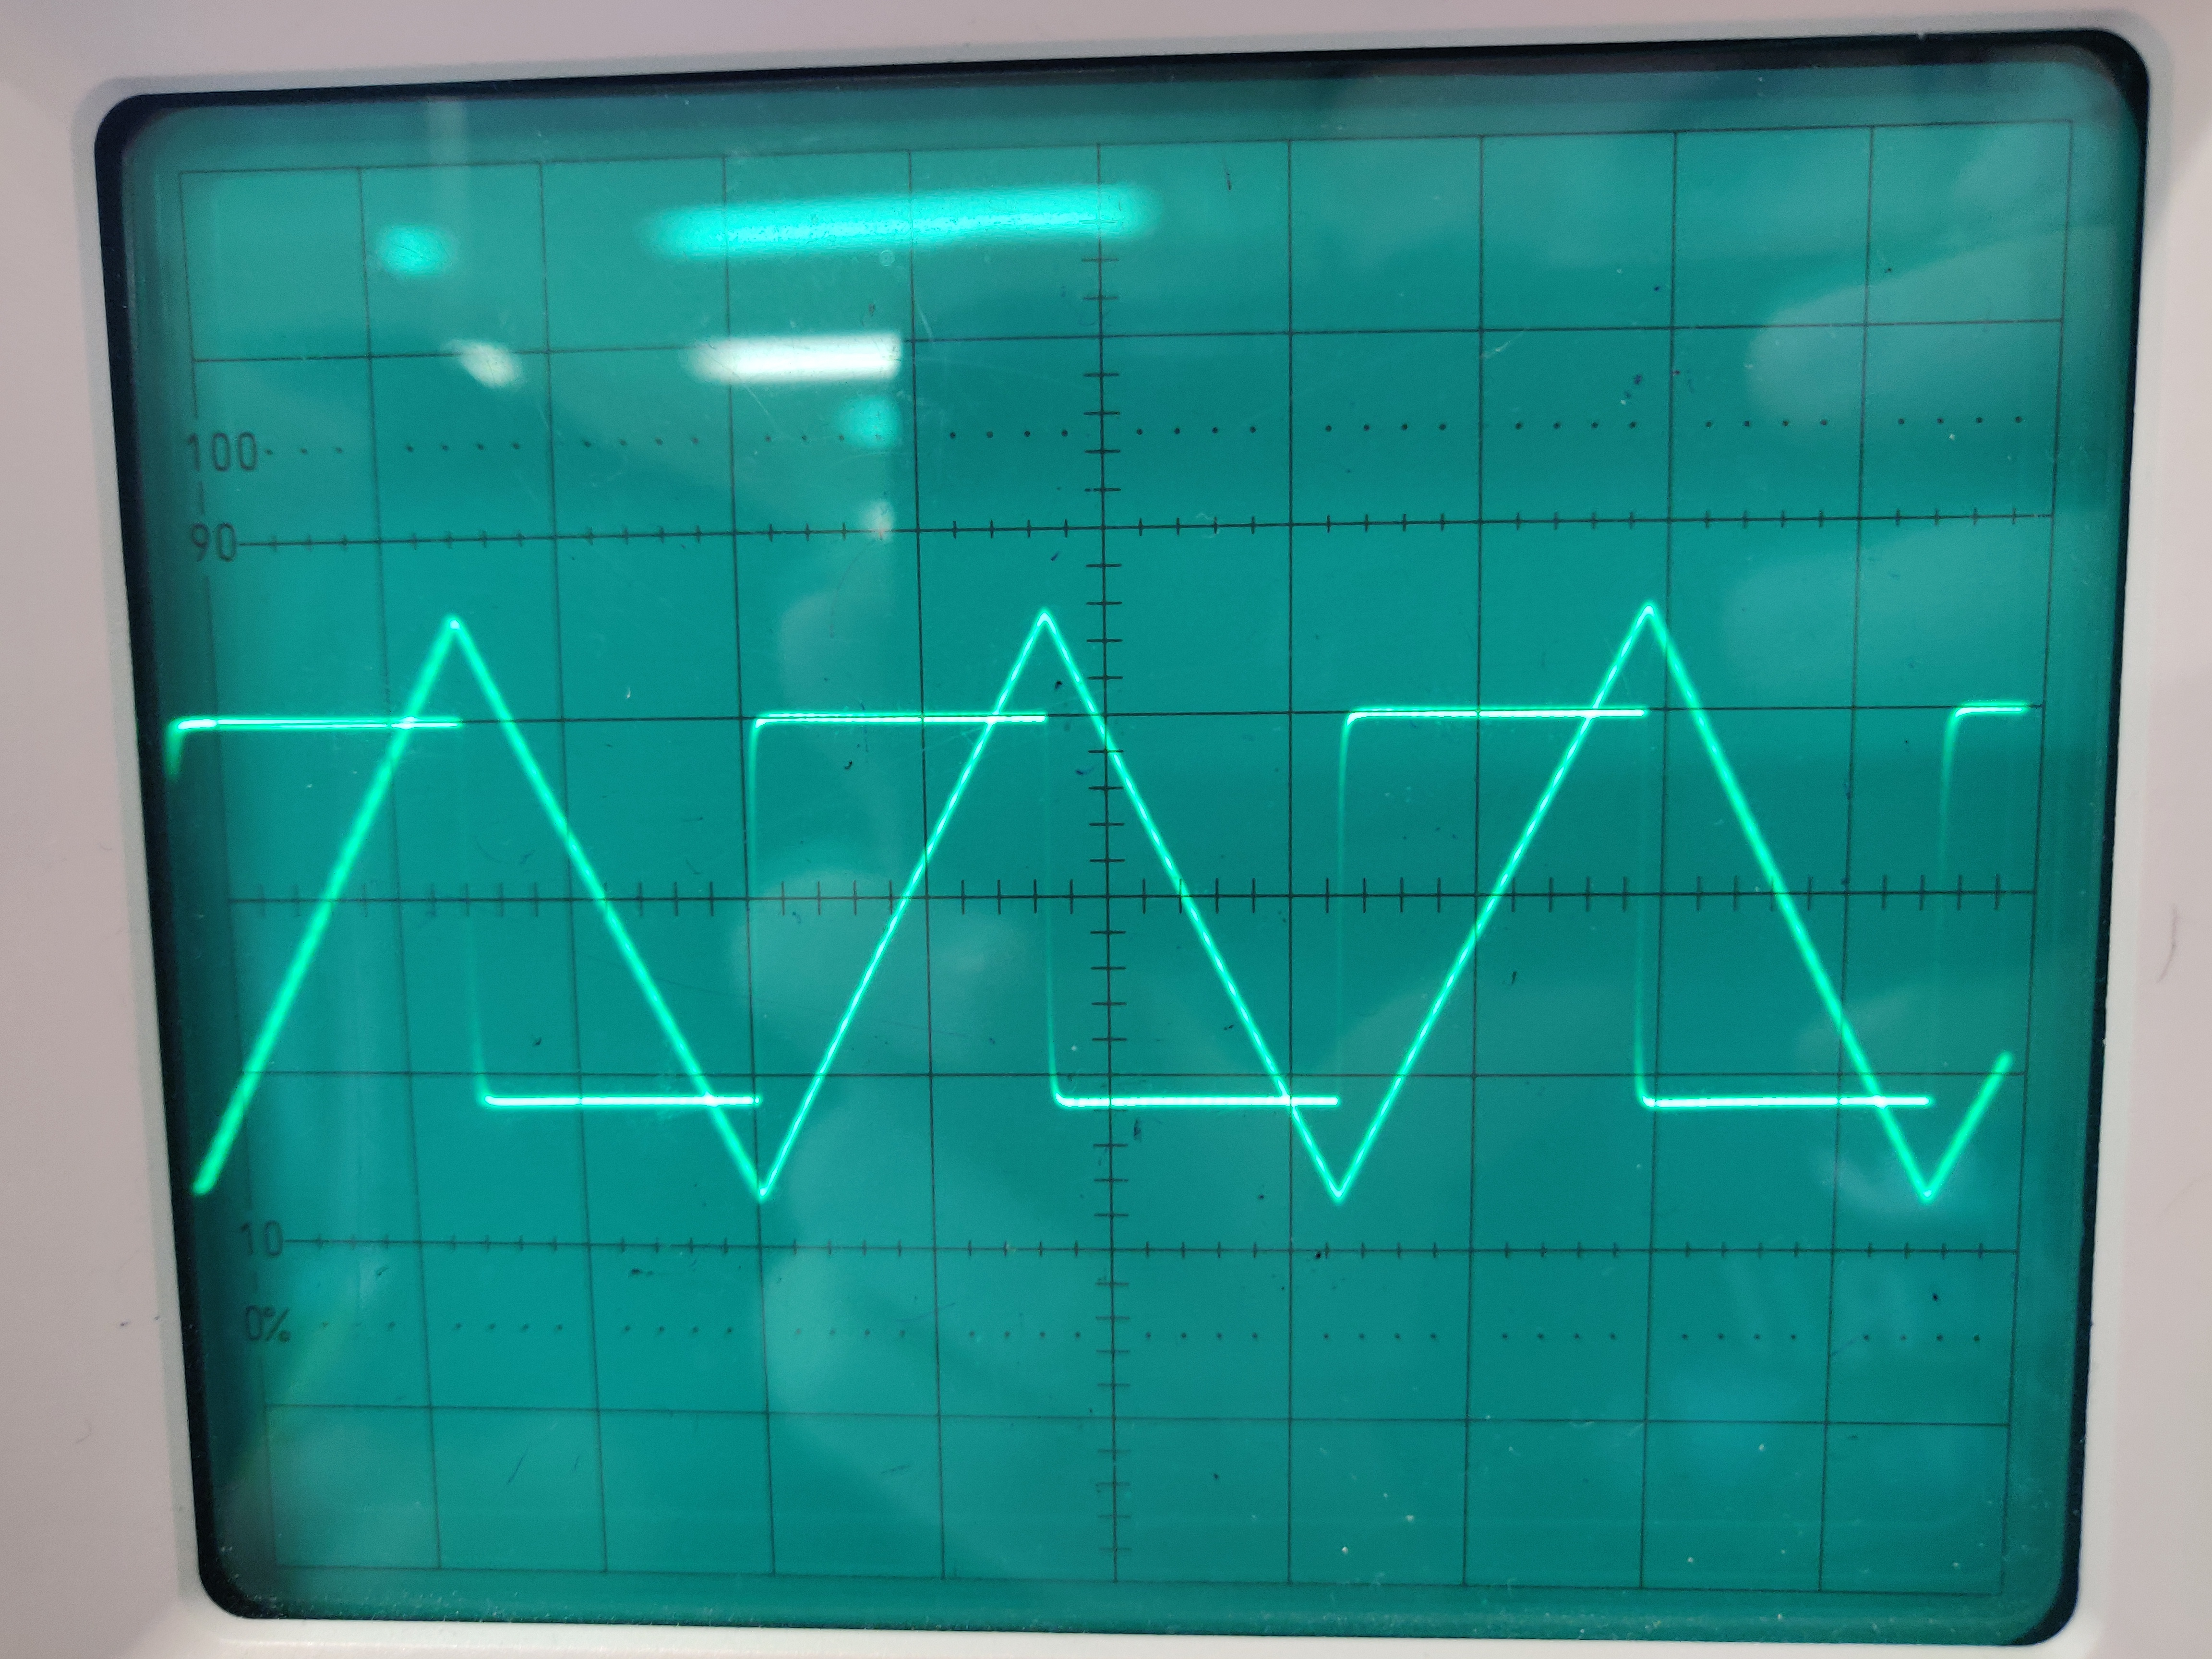
\includegraphics[width=\textwidth]{content/data/rechteck1.jpg}
            \caption[]%
            {{\small Rechteckschwingung}}    
            \label{fig:mean and std of net34}
        \end{subfigure}
        \quad
        \begin{subfigure}[b]{0.475\textwidth}   
            \centering 
            \includegraphics[width=\textwidth]{content/data/rechteck2.jpg}
            \caption[]%
            {{\small Offset-Spannung}}    
            \label{fig:mean and std of net44}
        \end{subfigure}
        \caption[]
        {\small Die verschiedenen Eingangssignale (Bildunterschriften) werden im RC-Glied integriert.} 
        \label{fig:integrabel}
    \end{figure}

    \begin{table}
        \centering
        \begin{tabular}{cc}
            \toprule
            Eingangsspannung $U$ & Kondensatorspannung $U_\text{c}$ \\
            \midrule
            $\sin(\omega t)$ & $-\cos(\omega t)$ \\
            $ax+b$ & $\frac{1}{2}ax^2+bx$ \\
            $a$ & $ax$ \\
            \bottomrule
        \end{tabular}
    \end{table}